\section{Design}
\subsection{Utseende}
Kodeordet for grafikken i Lille Promille er "oversiktlig". Derfor går vi for et rent utseende med få komponenter i hver side, slik at det ikke blir for mye rot. Hensikten er at man ønsker gjerne kun den relevante informasjonen i en slik app, spesielt når man er påvirket av alkohol. Nedtellingsklokken på forsiden er ganske stor for å fange oppmerksomheten, og videre er informasjon vist i rekkefølge nedover siden basert på viktighet. Dette design-prinsippet følger stort sett alle sider i appen for å gjøre opplevelsen mest behagelig som mulig for brukeren. Skjermbildene ovenfor demonstrerer dette.

Fargemessig har vi gått for nøytrale farger, med noe rødt og blått for å signalisere funksjonaliteten til brukeren. For eksempel en rød knapp for å signalisere at noe skal slettes, eller en blå tekst for å markere at den er interaktiv.

Videre har vi valgt å gruppere og abstrahere informasjon vekk fra første-sidene, slik at man ikke overvelder brukeren med informasjon. Et godt eksempel på dette er økt-historikken, da man kan velge å inspisere en spesifikk økt for å se mer informasjon om den økten. Dette er også et prinsipp som går gjennom hele appen. Appen benytter seg også av ikoner for å dirigere bruker i riktig retning og gi mer kontekst bak de interaktive elementene.

\subsection{Sider i Appen}
\subsubsection{Oversiktsside}
Et av de viktigste stedene i appen er oversiktssiden der all informasjon relatert til en \textit{økt} står oppsummert. Siden består av en nedtellingsklokke, en liste over hva man sist har drukket, og en knapp for å legge til en ny drukket enhet. 

Tanken her er at når brukeren begynner å drikke, legger de til en nydrukket enhet til listen vist på skjermen. I dette øyeblikket starter en ny økt, der nedtellingsklokken viser tiden det vil ta før man er \textit{kjørbar} basert på kjønn, vekt og høyde på brukeren. Dersom brukeren drikker enda en enhet, legges denne til i økten ved hjelp av knappen, og nedtellingen kalkuleres på nytt. Etter hvert som tiden går vil listen på oversiktssiden fylles opp med type enhet som ble konsumert, når den ble konsumert og hvor mye alkohol den inneholder. Under nedtellingsklokken vil det stå en tilnærmet verdi av den nåværende promillen i blodet til brukeren. 

Når nedtellingsklokken har nådd null sekunder, vil økten avsluttes og bruker vil være kjørbar. Denne økten vil derretter bli lagret, slik at man kan inspisere denne økten senere i en egen side med tidligere økter. 

\begin{figure}[H]
    \centering
    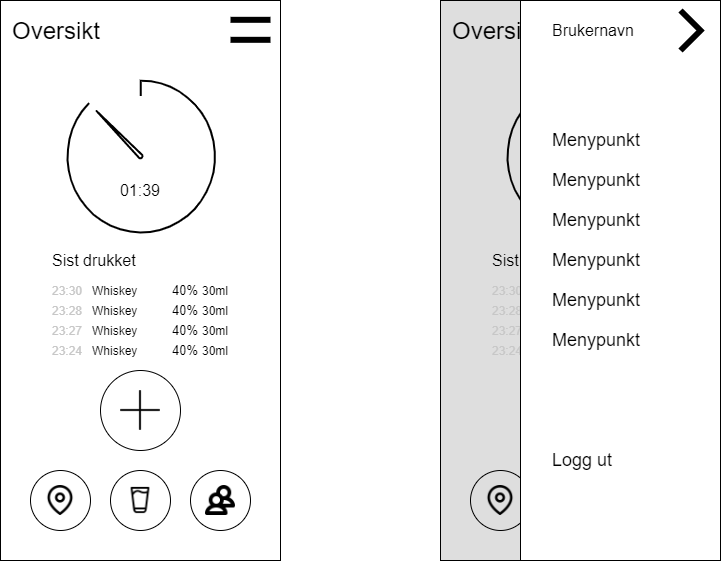
\includegraphics[scale=0.4]{images/lille_promille_frontpage.drawio.png}
    \caption{Til venstre er oversiktssiden med følgende elementer: Nedtellingsklokken, liste av nydrukkede enheter, en pluss-knapp og et navigasjonselement på bunnen. Når man trykker pluss knappen dirigeres man til enhetskatalogen, kan man velge en enhet man vil legge til i økten. Til høyre er det skisset en meny (navigation-drawer i Android studio) med menypunkter som man kan bruke til å navigere appen.}
\end{figure}

\subsubsection{Enhetskatalog}
Enhetskatalogen er en side med opplistning av alle definerte enheter i Appen, og brukes til å legge til enheter i løpet av en økt. Som ny bruker, vil det allerede ligge predefinerte enheter i listen som de kan bruke og gjøre endringer på. Ved behov kan nye enheter bli laget av brukeren gjennom pluss-knappen, da vil det komme opp en modal med noen tekst-felter. Her må brukeren beskrive navn på enheten, alkoholprosent og volum. For eksempel kan man lage en enhet som man kaller for "Whiskey Shot" med 40\% alkohol og 30ml volum. For å slette enheter trykker man på i-symbolet ved siden av navnet, og man blir sendt til en ny side med informasjon om den spesifikke enheten der man kan velge å slette enheten.

\begin{figure}[H]
    \centering
    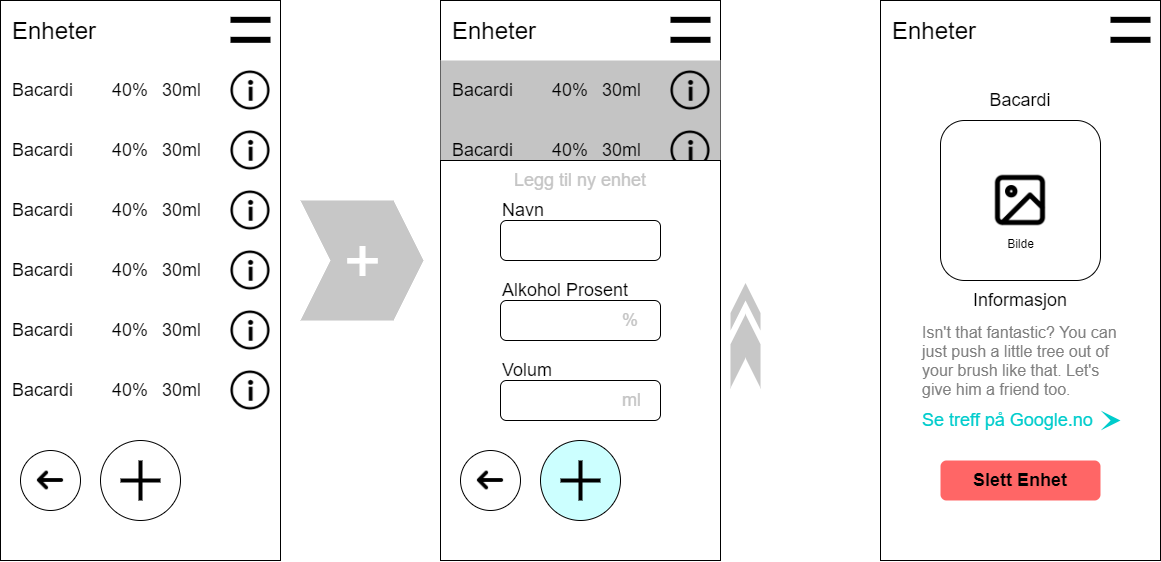
\includegraphics[scale=0.4]{images/lille_promille_unitcatalog.drawio.png}
    \caption{Enhetskatalogen: Listen til venstre består av tidligere definerte enheter. Det er denne siden man benytter når man skal legge til enheter i en økt, og det gjør man ved å trykke på navnet. Med pluss-knappen kan man legge til en ny enhet i listen, og med i-knappen kan man se mer informasjon om enheten. På informasjonssiden har man også valget å slette enheten fra listen.}
\end{figure}

\subsubsection{Innstillinger}
For å endre på noe med kontoen eller med appen går man til siden som heter "innstillinger". Her vil det være listet en rekke innstillinger gruppert etter konto, apputseende og generelle instillinger, som man kan endre på. Disse vil være knyttet opp til den spesifikke brukerkontoen som er logget inn. Når man endrer på en instilling oppdaters den lagrede instillingen umiddelbart.

\subsubsection{Venneside}
Vennesiden er der man kan legge til venner og se statusen på venner, som baserer seg på den nåværende økten. Man kan også sende emoji-meldinger til en venn i et chatrom. Dette er for å øke engasjementet ved å la brukerene kommunisere med hverandre, men de må være kreative i prosessen. Det kan bli interessant å se bruken av emojis når man er påvirket av alkoholen. 

\begin{figure}[H]
    \centering
    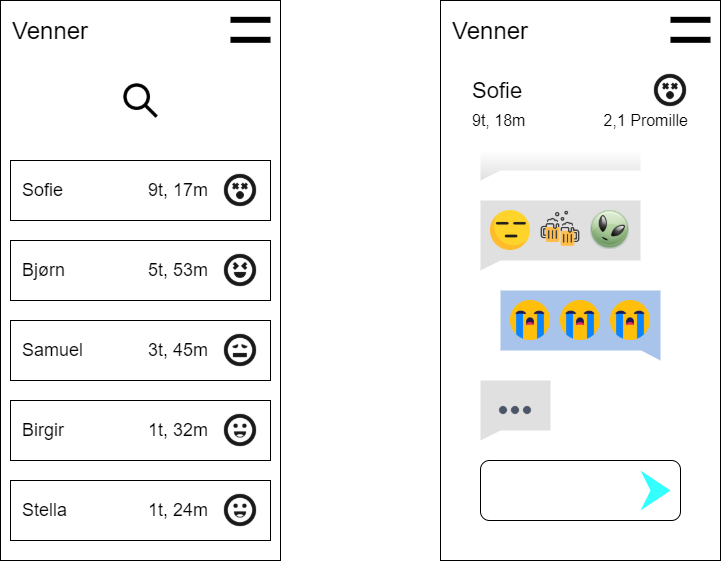
\includegraphics[scale=0.4]{images/lille_promille_friends.drawio.png}
    \caption{Til venstre er listen av venner. Det er tenkt at brukeren kan søke etter venner ved hjelp av forstørrelsesglasset og kunne sende de en venneforespørsel. Til høyre er en skisse av chat-funksjonen, hvor man kan sende emoji-meldinger til en venn. De kan også svare tilbake, og meldingene vil bli vist på siden sortert etter tid.}
\end{figure}

\subsubsection{Kartside}
Appen kommer med en kartside som bruker Google maps API-et. Dersom man er påvirket (En økt har begynt), vil kartet oppdatere hvor man har besøkt i perioden man er påvirket av alkohol. Hensikten med dette er å gi en geografisk oversikt over økten, slik at man vet hvor man har vært mens man drakk. Dette er en funksjon som mange studenter kan ha behov for, siden det ofte hender at de beveger seg rundt når de drikker.

\subsubsection{Innloggingsside}
Dersom man ikke er innlogget, eller man åpner Lille Promille appen for første gang, møter man en innloggingsside. Appen krever enten en e-mail og passord, eller en google-konto for å logge inn. Har man ikke noen av disse, kan man opprette en ny bruker ved å klikke "Opprett bruker" lenken på denne siden, da vil man bli ført til en ny side der man skriver ned en e-mail og et passord. Første gang man logger inn vil Appen spørre om navn, kjønn, vekt og høyde. Navnet er viktig i framvisningen av vennesiden, og de tre siste dataene brukes til beregning av promillen i blodet.

\subsubsection{Økthistorikk og Individuelle Økter}
Ettersom man gjennomgår flere og flere økter, vil de lagres ettersom i en egen historikkside for økter. Her vil man kunne se alle økter sortert etter kronologisk rekkefølge, og man kan inspisere hver individuelle økt ved å klikke på de. Når man gjør dette, åpnes en ny side med informasjon om den spesifikke økten.

\begin{figure}[H]
    \centering
    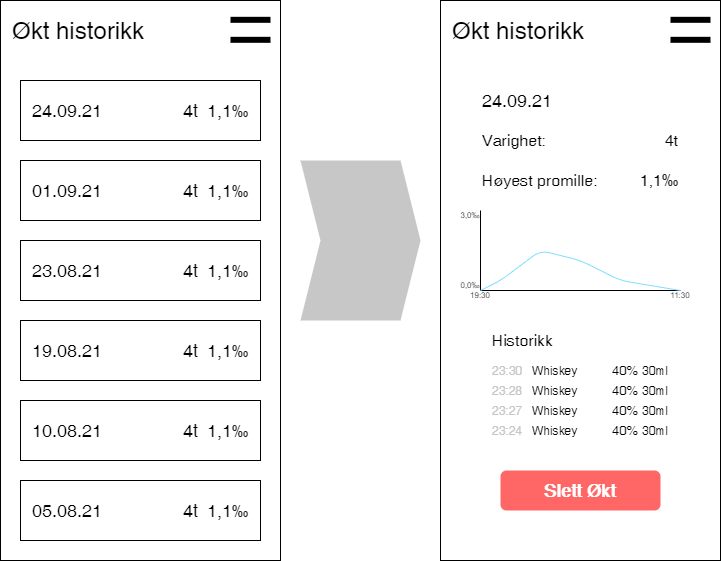
\includegraphics[scale=0.4]{images/lille_promille_sessions.drawio.png}
    \caption{Skisse som viser hvordan økt-historikksiden kan se ut. Her kan man inspisere hver individuelle økt og få utdypet data om hver økt. Det er også mulig å slette en økt.}
\end{figure}